\documentclass[12pt,a4paper]{article}
% Essential packages
\usepackage[utf8]{inputenc} % Character encoding
\usepackage{graphicx} % For images
\usepackage{amsmath} % For mathematical formulas
\usepackage{hyperref} % For hyperlinks
\usepackage{enumitem}
\usepackage{float} % For controlling figure placement
% Listings for code
\usepackage{listings}
\lstset{
 language=C,
 basicstyle=\ttfamily\small,
 numbers=left,
 frame=single,
 breaklines=true,
}
% Tighten space before sections
\usepackage{titlesec}
\titlespacing*{\section}{0pt}{0.5em}{0.5em}
\titlespacing*{\subsection}{0pt}{0.3em}{0.3em}
\setlength{\parindent}{0pt}

% Document metadata
\title{\textbf{Documentation Cellular Automats (Assignment 15)}}
\author{Mario Neuner, Christoph Bichlmeier, Jakob Guentner\\Leander Decristoforo}
\date{\today}
\begin{document}
\maketitle
\vspace{5cm}
\tableofcontents
\pagebreak


% Problem 1
\section{Part A: One Dimensional Cellular Automats}
\vspace{1cm}


\subsection{Task}
The task involves implementing a one-dimensional cellular automaton system that 
evolves through discrete time steps based on predefined rules. The automaton consists 
of a linear array of cells, each in state 0 or 1, where the next state is determined by 
a cell's current state and its immediate neighbors. The system must support four specific 
rules (22, 106, 187, 214) and handle two initialization modes: a determined start with a 1 
in the middle and zeros around and a random configuration. The program takes two command-line 
arguments, N for grid size and M for the number of time iterations and outputs the automaton's 
state after each iteration. These results can then be visualized using a separate plotting tool.
\newline

\vspace{1cm}


\subsection{Idea}
This project is built around a modular and rule-driven approach to simulating cellular automata. 
At the heart of the system is a structure called “cellauto”, which holds the key components of the 
simulation. It holds the current state of the grid, stored as a character array, the rule being applied 
encoded as an 8-bit pattern and parameters like the grid size N and number of iterations M.
\newline
The rules themselves are defined using arrays of eight characters, where each position corresponds to 
one of the possible neighborhood cell configurations (e.g., the pattern “111” maps to index “0”). During 
the simulation, the system updates the grid in steps. For each cell, considering its left, center, and right 
neighbors, wrapping around at the edges, determining the corresponding rule index, and updating the cell’s 
state based on the rule.
\newline
There are two modes of initialization implemented, one is determined, starting with a 
single 1 in the center and zeros around, and one random. 
The results of each simulation are saved in a format designed for easy visualization. 
Each line in the output file represents the complete state of the cells at a given time step.
\newline

\vspace{1cm}


\subsection{Implementation}
\subsection*{\small Data Structures and Rule Encoding}
At the core of the system is the \texttt{cellauto}-struct, defined in \texttt{structs.h}. This struct houses all the 
parameters and data needed to run a simulation, including the current state of the grid, the active rule, 
the simulation data, and the mode of initialization:
\newline
The rule definitions themselves are declared as global constants in \texttt{structs.h} and initialized in \texttt{structs.c}. 
Each rule is represented as an array of eight characters \texttt{(e.g., RULE\_22)}, corresponding to the eight possible 
arrangement of three cells. These arrays are indexed from 0 to 7, where each index corresponds to a specific 
neighborhood pattern. For instance, \texttt{Rule\_22 = \{0,0,0,1,0,1,1,0\}} defines the rule's response to configurations 
ranging from 111 with index 0 to 000 with index 7. 
\newline

\subsection*{\small State Management and Rule Application}
The evolution of the automaton is made by functions implemented in \texttt{cell.c}. Where two initialization modes are used. 
One Deterministic via \texttt{reset(cellauto *c)}, which sets a single active cell (1) at the center of the grid, and the other 
one Random via \texttt{randomize(cellauto *c)}, which assigns each cell a 0 or 1 at random, using \texttt{srand(time(NULL))}.
\newline
The key function that does the state transitions is \texttt{apply\_rule(cellauto *c, char *next\_state)}. For each cell in the 
current state array, the function considers its left, center, and right neighbors. These three bits form a 3-digit 
binary number, which is converted into a decimal index between 0 and 7. This index is then used to look up the new 
state in the rule array. For example, the neighborhood 0 1 0 corresponds to binary 010, or decimal 2. Applying \texttt{Rule\_22}, 
the next state is retrieved via \texttt{RULE\_22[2]}, which equals to 0.
\newline

\subsection*{\small Simulation Flow and Execution}
The entry point of the program is \texttt{main()} in \texttt{1d\_states.c}. It expects two command-line arguments: the grid size \texttt{N} and the 
number of iterations \texttt{M}. It starts with the input handling, where the program verifies the validity of user input and 
allocates memory for a \texttt{cellauto} instance and its state array. It returns an error message if memory allocation fails or 
if the inputs are invalid.
\newline
First it runs the deterministic Initialization where the grid is initialized using \texttt{reset()}. The simulation runs for each 
of the four predefined rules (\texttt{RULE\_22}, \texttt{RULE\_106}, \texttt{RULE\_187}, \texttt{RULE\_214}), updating the \texttt{rule} pointer and \texttt{rule\_name} along the 
way. For each rule, the \texttt{steps()} function is called to run the system for the given number of iteration steps. At each step, 
the full state is saved in a file named \texttt{1d\_states/1d\_rule\_<Regel>.txt}, where \texttt{<Regel>} is the rule number.
\newline
For Random Initialization Phase the random number generator initializes a new starting grid. For each rule, the state is 
randomized in \texttt{randomize()}, and the simulation is repeated as explained previously. Each rule’s results under random initial 
conditions are also saved to the file named 
\newline
\texttt{1d\_states/1d\_rule\_<Regel>\_random.txt} for comparison.
\newline

\vspace{1cm}


\subsection{Output}
The program generates two types of output:
\newline
\vspace{0.1 cm}

First a \texttt{Text File} for each rule (e.g., \texttt{1d\_rule\_22.txt}) recording the grid state per iteration, 
space-separated (e.g., \texttt{0 0 1 1 0 0 0}). 
These files are saved in the \texttt{1d\_states} directory, where they are created automatically.
\newline
There is also a \texttt{Visualization} created with the \texttt{plot\_1d} tool reading the created files and producing 
PNG images (e.g., \texttt{1d\_plots/1d\_rule\_22.png}) using \texttt{gnuplot}. Each image depicts the automaton's evolution 
over time, with rows representing iterations and black/white pixels for 1/0 states.
\newline
\vspace{0.1 cm}

\begin{enumerate}[label=\roman*.]
    \item 
    To use the system, you have to compile by using the \texttt{Makefile} with the command \texttt{"make"}.
    \newline
    \vspace{0.1 cm}

    \item 
    To run the simulation, use the command: \texttt{"./1d\_states N M"} (e.g., \texttt{201 100}).
    \newline
    \vspace{0.1 cm}

    \item 
    To generate the plots, use the command: \texttt{"./plot\_1d 22"} (e.g., for \texttt{Rule\_22}).
\end{enumerate} 

\vspace{3.5 cm}
\texttt{Examples: Here with initial state of 1 in the middle.}  
\newline


% Picture of rule 22
\begin{figure}[H]
    \centering
    \fbox{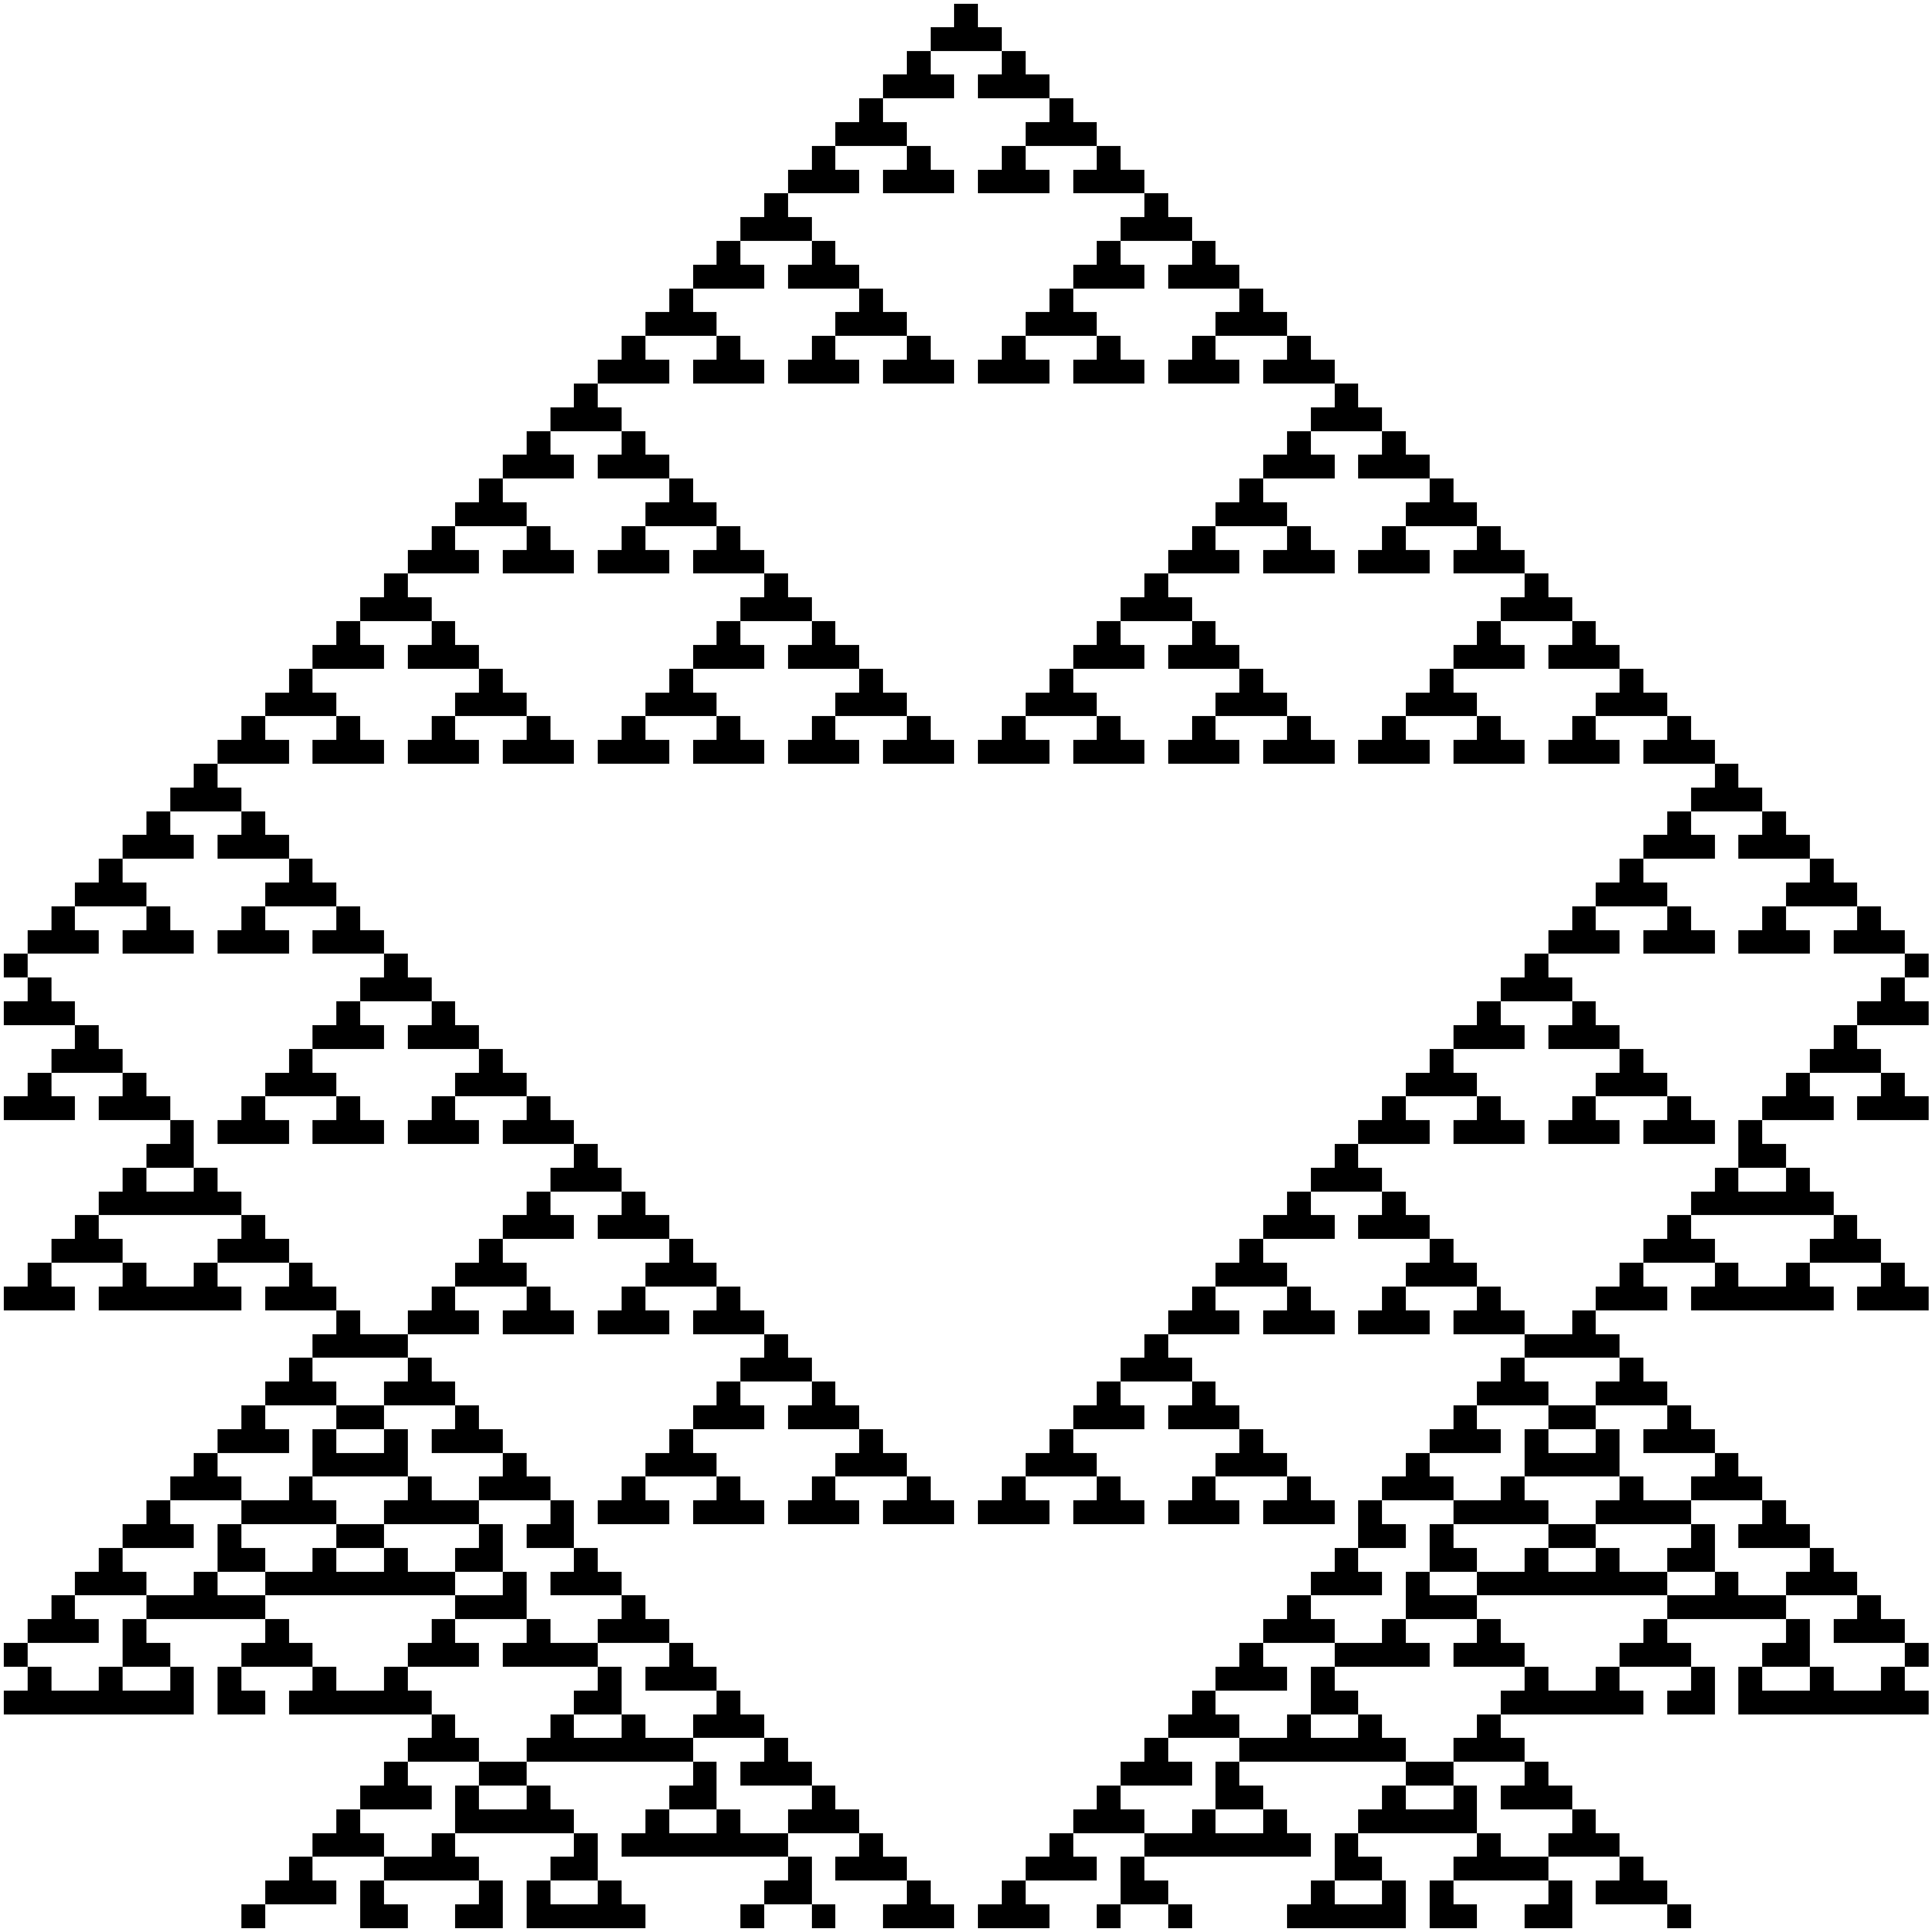
\includegraphics[width=8cm, height=8cm]{1d_plots/1d_rule_22.png}}
    \caption{Rule\_22; N=151, M=151}
    \label{fig:your_label}
\end{figure}

\vspace{0.5cm}

% Picture of rule 22
\begin{figure}[H]
    \centering
    \fbox{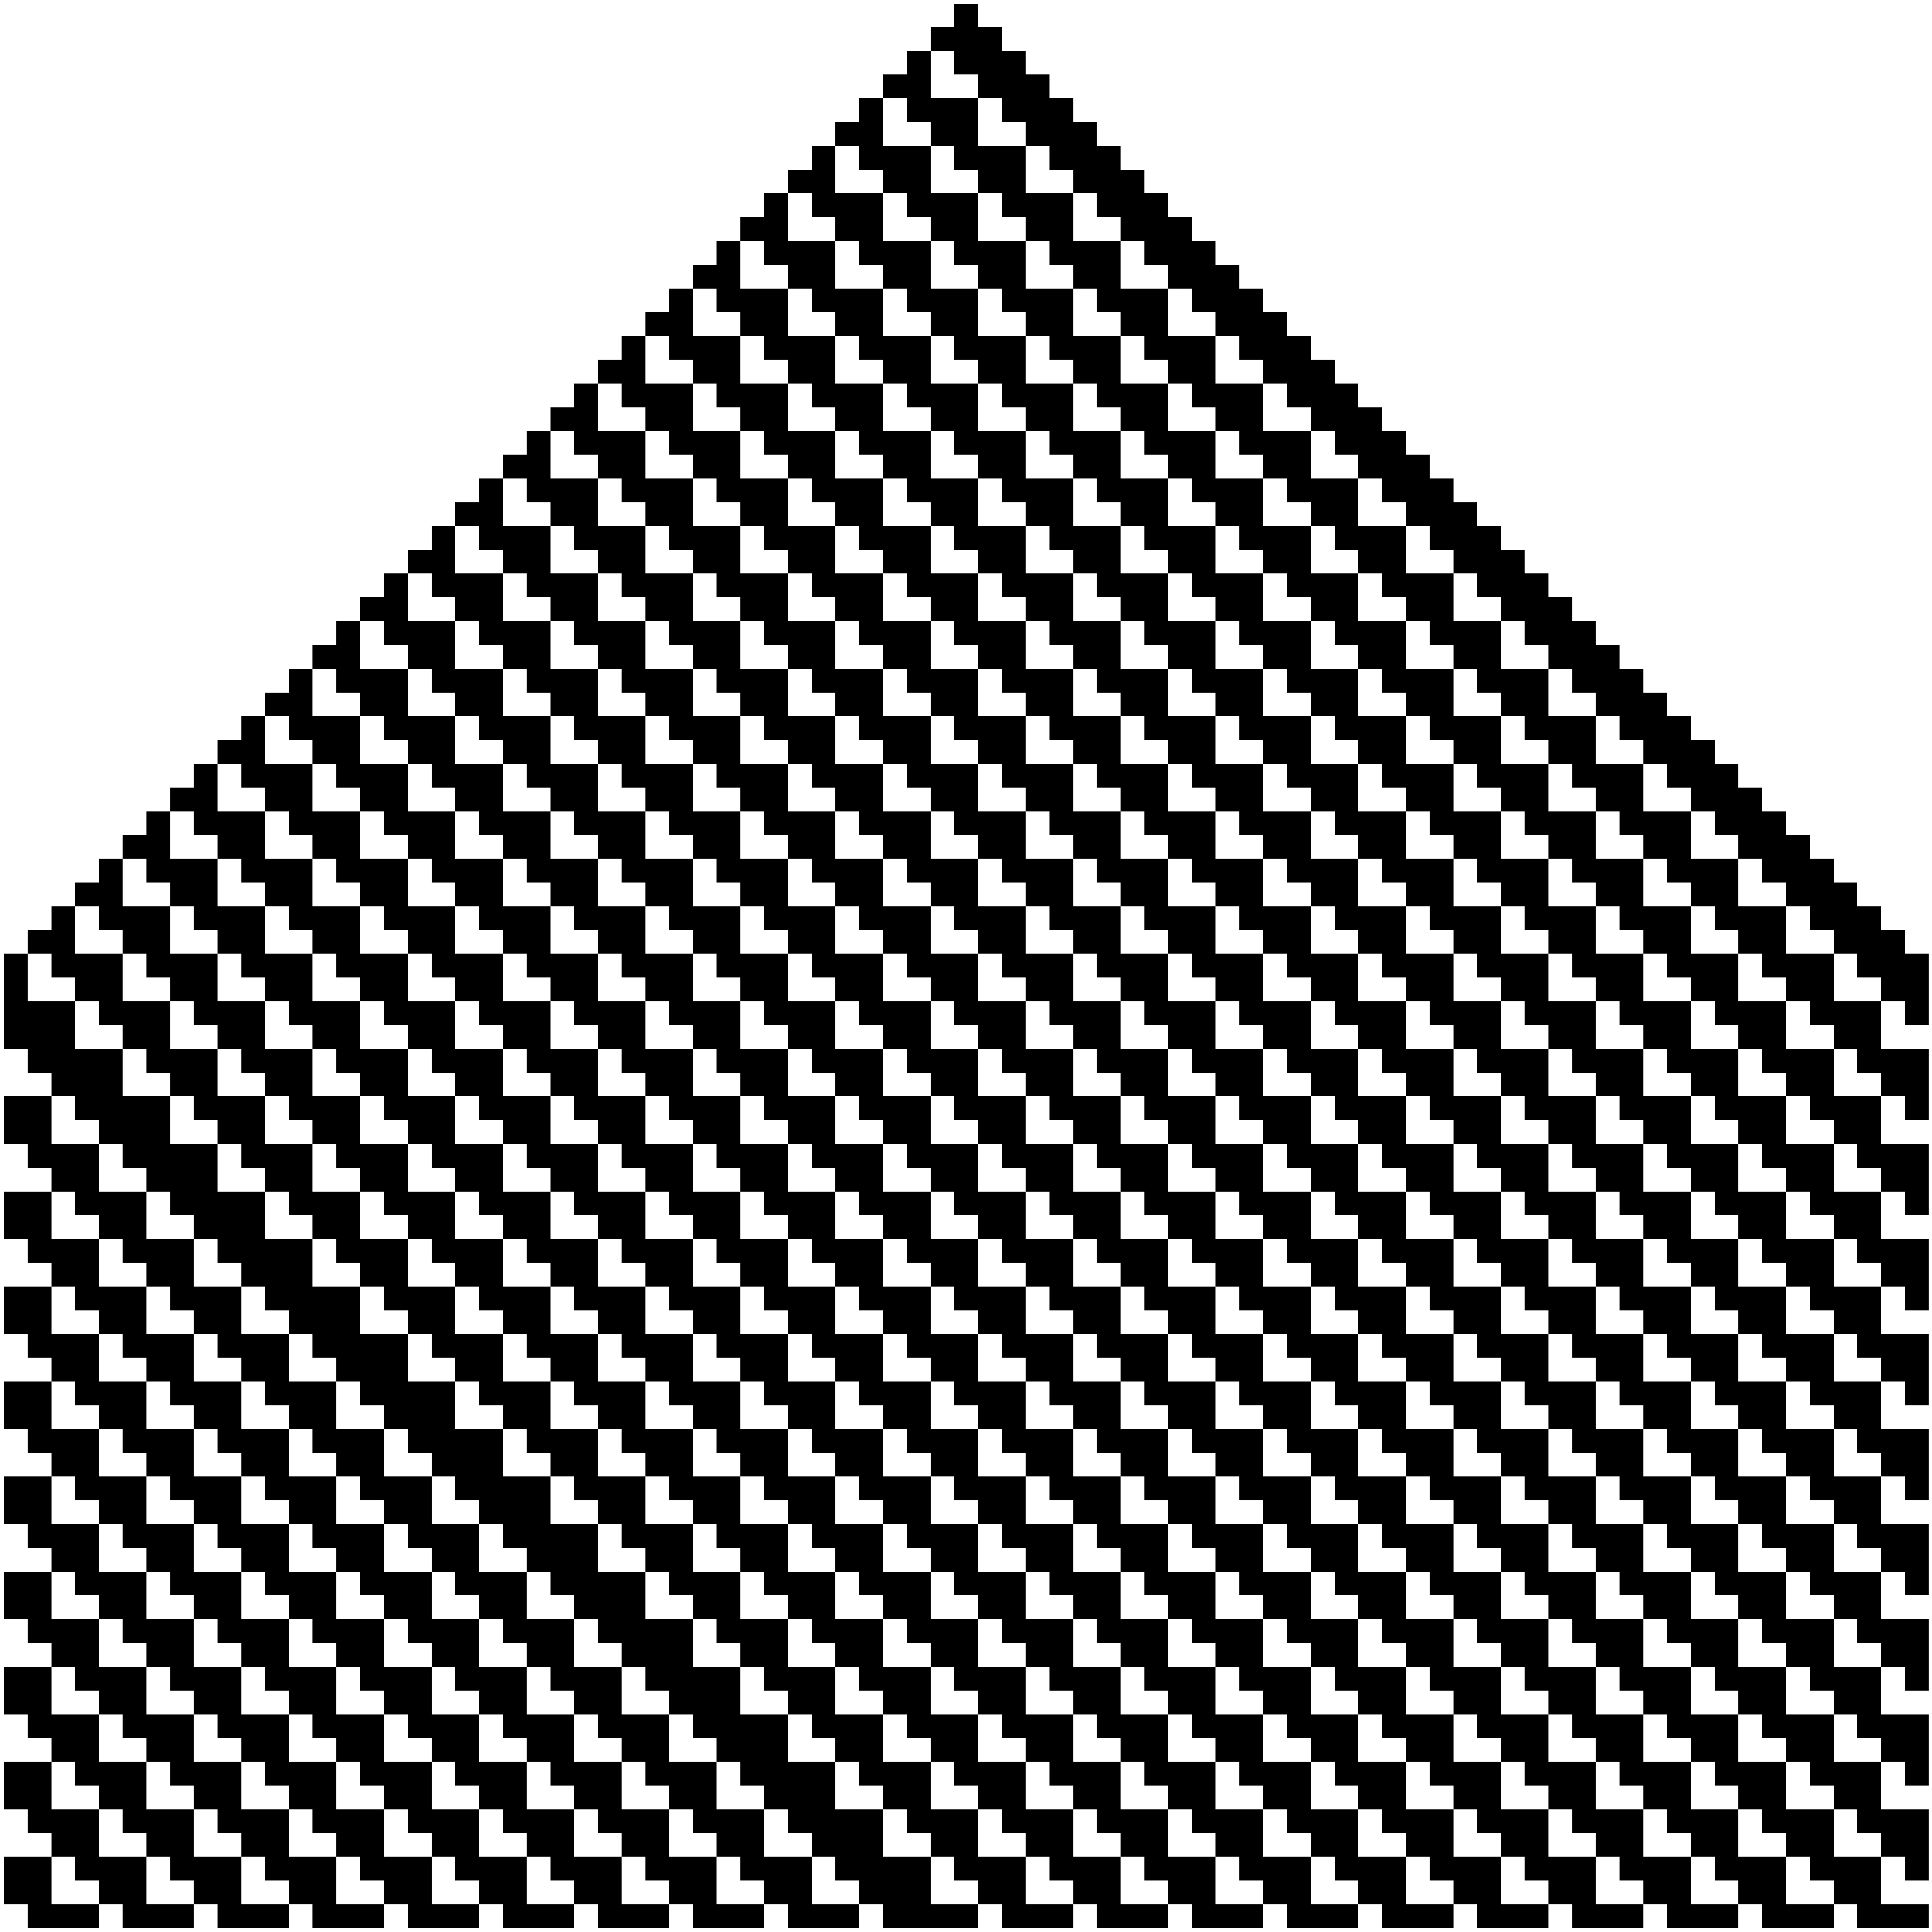
\includegraphics[width=8cm, height=8cm]{1d_plots/1d_rule_214.png}}
    \caption{Rule\_214; N=151, M=151}
    \label{fig:your_label}
\end{figure}

\vspace{1cm}





% Problem 2
\section{Part B}


\vspace{1cm}

\subsection{Idea}


\vspace{1cm}

\subsection{Implementation}


\vspace{1cm}

\subsection{Output}
\texttt{The program compiles with "gcc -Wall -Wextra -Werror -Wpedantic -std=c18 rakete.c -o rakete".}
When running \texttt{./rakete <masse\_leer> <masse\_treibstoff> <geschwindigkeit\_treibstoff> <massenverlustrate\_treibstoff>} 
you get the output:

\vspace{1cm}



\vspace{1cm}


% Code for all parts
\section{Appendix: Code}

\subsection{Part A: Main}
% Code listing with even smaller font size
\begin{lstlisting}[caption={Main (1d\_states.c)},label={lst:p7001},basicstyle=\ttfamily\tiny]
    #include <stdio.h>
    #include <stdlib.h>
    #include <string.h>
    #include <time.h>

    // Own headers with function declarations, structs etc. 
    #include "structs.h"
    #include "cell.h"
    #include "stepcom.h"


    int main (int argc, char *argv[]) {
        if (argc != 3) {
            fprintf(stderr, "Usage: %s <n> <m>\n", argv[0]);
            return 1;
        }

        // User input for size and iterations
        int size = atoi(argv[1]);
        if (size <= 0) {
            fprintf(stderr, "Error: Size must be a positive integer.\n");
            return EXIT_FAILURE;
        }
        int iterations = atoi(argv[2]);

        // Initialize state
        cellauto *cell = malloc(sizeof(cellauto));
        if (!cell) {
            fprintf(stderr, "Error: Memory allocation failed.\n");
            return EXIT_FAILURE;
        }
        cell->state = malloc(size * sizeof(char));
        if (!cell->state) {
            fprintf(stderr, "Error: Memory allocation for state failed.\n");
            free(cell);
            return EXIT_FAILURE;
        }
        cell->rule = NULL; 
        cell->rule_name = 0;
        cell->rand = false;
        cell->iterations = iterations;
        cell->size = size;


        reset(cell); // Initialize state with a single '1' in the middle
        cell->rule = RULE_22;
        cell->rule_name = 22;

        // Compute steps for not random initial condition
        steps(cell);
        reset(cell); 
        cell->rule = RULE_106;
        cell->rule_name = 106;

        steps(cell);
        reset(cell); 
        cell->rule = RULE_187;
        cell->rule_name = 187;

        steps(cell);
        reset(cell); 
        cell->rule = RULE_214;
        cell->rule_name = 214;

        steps(cell);
        reset(cell); 


        // Now random states
        cell->rand = true;

        // Set random initial state
        srand(time(NULL)); // Seed for random number generation
        randomize(cell);
        cell->rule = RULE_22;
        cell->rule_name = 22;

        // Compute steps for random initial condition
        steps(cell);
        randomize(cell); 
        cell->rule = RULE_106;
        cell->rule_name = 106;

        steps(cell);
        randomize(cell); 
        cell->rule = RULE_187;
        cell->rule_name = 187;

        steps(cell);
        randomize(cell); 
        cell->rule = RULE_214;
        cell->rule_name = 214;

        steps(cell);

        // Free allocated memory
        free(cell->state);
        free(cell);

        return EXIT_SUCCESS;
    }
\end{lstlisting}


\end{document}